\documentclass[10pt,a4paper]{article}

% ------------------------------------------------------------------
% InJET (KEC Journal) paper format: single column, A4, Times New Roman,
% 1in top/bottom/right margins, 1.25in left margin, 1.15 body line spacing.
% ------------------------------------------------------------------
\usepackage[top=1in,bottom=1in,left=1.25in,right=1in]{geometry}
\usepackage{mathptmx} % Times-compatible text and math font
\usepackage{amsmath}
\usepackage{amssymb}
\usepackage{graphicx}
\usepackage{booktabs}
\usepackage{caption}
\usepackage{titlesec}
\usepackage{setspace}
\usepackage{enumitem}
\usepackage{multirow}
\usepackage[hidelinks]{hyperref}

% Section headings: bold, Arabic-numbered, left justified (Sec. 1.5 of template)
\titleformat{\section}{\bfseries\fontsize{10}{12}\selectfont}{\thesection.}{0.6em}{}
% Sub-section headings: bold italic, numbered 1.1, 1.2, left justified
\titleformat{\subsection}{\bfseries\itshape\fontsize{10}{12}\selectfont}{\thesubsection.}{0.6em}{}
\titleformat{\subsubsection}{\bfseries\itshape\fontsize{10}{12}\selectfont}{\thesubsubsection.}{0.6em}{}
\titlespacing*{\section}{0pt}{1.2em}{0.6em}
\titlespacing*{\subsection}{0pt}{1em}{0.4em}
\titlespacing*{\subsubsection}{0pt}{0.8em}{0.3em}

% Table captions above, figure captions below, both 8pt, centered (Sec. 1.2, 2)
\captionsetup[table]{position=above,font=scriptsize,labelsep=period,justification=centering}
\captionsetup[figure]{position=below,font=scriptsize,labelsep=period,justification=centering}

\setstretch{1.15} % body text line spacing

% Tighter float/caption spacing to fit the 8-page limit without changing margins or body spacing
\setlength{\textfloatsep}{6pt plus 1pt minus 2pt}
\setlength{\floatsep}{4pt plus 1pt minus 1pt}
\setlength{\intextsep}{5pt plus 1pt minus 1pt}
\setlength{\abovecaptionskip}{3pt}
\setlength{\belowcaptionskip}{2pt}
\setlength{\abovedisplayskip}{4pt plus 1pt minus 1pt}
\setlength{\belowdisplayskip}{4pt plus 1pt minus 1pt}
\setlength{\abovedisplayshortskip}{2pt plus 1pt minus 1pt}
\setlength{\belowdisplayshortskip}{2pt plus 1pt minus 1pt}

\hypersetup{
    pdftitle={A Hybrid CNN-TCN Deep Learning Architecture for El Nino-Southern Oscillation Forecasting},
    pdfauthor={Biraj Adhikari, Raman Shrestha, Rojin Dhami, Sandeep Khadka},
    pdfsubject={El Nino-Southern Oscillation forecasting with deep learning},
    pdfkeywords={ENSO; El Nino; deep learning; CNN; TCN; spatiotemporal forecasting; sea surface temperature; climate forecasting}
}

\begin{document}
\pagestyle{plain}

% ------------------------------------------------------------------
% Title, Authors, Affiliations (Sec. "Structure": Title, Authors,
% Affiliations, Abstract, Keywords, Main text, Acknowledgements,
% References, Appendix)
% ------------------------------------------------------------------
\begin{center}
{\fontsize{17}{20}\selectfont\bfseries A Hybrid CNN-TCN Deep Learning Architecture for El Ni\~no--Southern Oscillation Forecasting}

\vspace{0.5em}
{\fontsize{13}{16}\selectfont Biraj Adhikari$^{1}$, Raman Shrestha$^{1,\ast}$, Rojin Dhami$^{1}$, Sandeep Khadka$^{1}$}

\vspace{0.25em}
{\fontsize{8}{10}\selectfont
$^{1}$Department of Electronics and Computer Engineering, Thapathali Campus, Institute of Engineering, Tribhuvan University, Kathmandu, Nepal\\
$^{\ast}$Corresponding author: raman.shrestha@example.edu.np}
\end{center}

\vspace{0.3em}
\noindent\textbf{Abstract:} Dynamical forecast models of the El Ni\~no--Southern Oscillation (ENSO) lose skill beyond a 6--9 month horizon due to the spring predictability barrier. This paper presents a hybrid Convolutional Neural Network--Temporal Convolutional Network (CNN-TCN) that forecasts the Ni\~no 3.4 index at 3- and 6-month lead times directly from ERA5 and ORAS5 reanalysis fields (1980--2025): the CNN component extracts spatial sea-surface-temperature and ocean-heat-content gradient patterns from each monthly snapshot of the tropical Pacific, while the TCN component, using dilated causal convolutions, models their evolution across a 12-month input window without any explicit feature selection. On a chronological train (1980--2018), validation (2019--2022), and test (2023--2026) split, the CNN-TCN achieves a test RMSE of 0.3781\textdegree C and a Pearson correlation of 0.9474 at 3-month lead, and remains usable at 6-month lead (RMSE 0.6806\textdegree C, $r=0.8256$); a 5-member ensemble confirms stable skill (mean test correlation $0.9195\pm0.0167$). To contextualize this result, the CNN-TCN is benchmarked against the stronger of two Mutual Information Feature Selection (MIFS)-based XGBoost baselines developed on the same data: a 500-feature, correlation-approximated MIFS configuration dominated by upper-300 m ocean heat content, which reaches a test RMSE of 0.5299\textdegree C and correlation of 0.9207 but exhibits a large train-test generalization gap (train $R^2=1.000$ vs.\ test $R^2=0.5805$). Relative to this best baseline, the CNN-TCN reduces test RMSE by 55.8\% and shrinks the train-test RMSE gap by 96\%, showing that preserving the spatial topology of climate reanalysis fields through convolutional and dilated temporal convolutions yields substantially better generalization and amplitude fidelity than flattened-tensor, feature-selected gradient boosting for ENSO forecasting.

\vspace{0.3em}
\noindent\textbf{Keywords:} El Ni\~no--Southern Oscillation, ENSO, deep learning, convolutional neural network, temporal convolutional network, spatiotemporal forecasting, sea surface temperature, climate forecasting.

\vspace{0.4em}

\section{Introduction}

\subsection{Background}
The El Ni\~no--Southern Oscillation (ENSO) is the dominant mode of interannual climate variability, influencing weather patterns worldwide through coupled ocean-atmosphere interactions in the tropical Pacific \cite{ham2019}. ENSO cycles between warm (El Ni\~no) and cool (La Ni\~na) phases, driven primarily by anomalies in Sea Surface Temperature (SST) across the equatorial Pacific Ocean, with far-reaching teleconnections that affect precipitation, temperature, and extreme weather events across multiple continents.

Traditional dynamical climate models, such as General Circulation Models (GCMs), provide seasonal ENSO forecasts but face limitations in prediction skill beyond 6--9 months due to the ``spring predictability barrier,'' a phenomenon in which forecast initialization errors grow rapidly during boreal spring \cite{mahesh2024}. Recent advances in deep learning have demonstrated superior forecasting skill at longer lead times by extracting complex spatiotemporal patterns from large reanalysis archives \cite{ham2019, mahesh2024}, using architectures such as Convolutional Neural Networks (CNNs) and Long Short-Term Memory (LSTM) networks to capture nonlinear dynamics that classical statistical methods and dynamical models struggle to represent.

\subsection{Motivation and problem statement}
Despite significant progress in ENSO forecasting using deep learning, existing approaches face a recurring limitation: models that flatten spatially gridded reanalysis fields into tabular feature vectors -- a necessary step for classical machine learning regressors -- discard the spatial topology of the climate system, so that neighboring, highly autocorrelated grid cells must be pruned via feature selection before a tabular model can be trained without severe overfitting. Published comparisons also rarely quantify, on a single consistent chronological data split, how much predictive skill and generalization capability is gained by preserving that spatial structure end-to-end, relative to even the best available feature-selected tabular baseline.

This paper addresses these gaps by designing and training a hybrid CNN-TCN architecture that consumes the full 4-D spatiotemporal tensor of tropical Pacific reanalysis fields end-to-end, without any feature reduction step, and forecasts the Ni\~no 3.4 index at both 3- and 6-month lead times. To rigorously establish the value of this spatiotemporal approach, the CNN-TCN is benchmarked against the stronger of two independently developed Mutual Information Feature Selection (MIFS) pipelines for a tabular XGBoost baseline, on identical training, validation, and test partitions.

\subsection{Objectives and contributions}
The primary objectives of this work are:
\begin{itemize}[leftmargin=1.4em]
\item To construct a validated, physically consistent 12-month sliding-window tensor of tropical Pacific SST, sea level pressure, wind stress, and subsurface ocean heat content anomalies from ERA5 and ORAS5 reanalysis data (1980--2025) for ENSO forecasting.
\item To design and train a CNN-TCN architecture that forecasts the Ni\~no 3.4 index at 3- and 6-month lead times directly from the unflattened spatiotemporal tensor, with no explicit feature selection, and to establish its robustness via a 5-member training ensemble.
\item To develop two candidate MIFS feature-selection pipelines for a tabular XGBoost baseline, and to report only the stronger of the two as the benchmark against which the CNN-TCN's improvement is quantified under an identical chronological evaluation protocol.
\end{itemize}

The remainder of this paper is organized as follows. Section 2 reviews related deep learning approaches to ENSO forecasting. Section 3 describes the data sources and preprocessing pipeline. Section 4 presents the CNN-TCN architecture and the best-performing MIFS-XGBoost baseline against which it is benchmarked. Section 5 details the experimental setup. Section 6 reports and analyzes the results, and Section 7 discusses the findings before Section 8 concludes with limitations and future work.

\section{Related work}

Table \ref{tab:litreview} summarizes representative deep learning approaches to ENSO forecasting. Ham et al.\ \cite{ham2019} pre-trained a CNN on CMIP5 simulations and fine-tuned it on SST, ocean heat content, and sea level pressure reanalysis maps, reaching 0.65 correlation at 17-month lead but with reduced La Ni\~na skill and no uncertainty quantification. Dijkstra et al.\ \cite{dijkstra2019} combined a convolutional autoencoder with an LSTM over its latent SST representation, achieving competitive 6--12 month skill with physically interpretable latent dimensions. Mahesh et al.\ \cite{mahesh2024} embedded recharge-discharge and delayed-oscillator theory as structural priors in a Deep Echo State Network, exceeding 0.5 correlation at 18-month lead with far fewer trainable parameters.

Ye et al.\ \cite{ye2024} developed ResoNet, a residual-attention architecture over SST, ocean heat content, and wind stress that exceeds 0.7 correlation at 12-month lead and remains useful beyond 18 months, with ensemble-based uncertainty estimation. Dutta et al.\ \cite{dutta2024} applied Random Forest, Gradient Boosting, and SVM classifiers to categorical seasonal precipitation and temperature anomalies from ENSO indices, reporting 70--82\% classification accuracy at 2--3 month lead. Relative to this body of work, the present study contributes an end-to-end spatiotemporal CNN-TCN model whose improvement is quantified, on a single consistent chronological split, against the stronger of two independently developed mutual-information-feature-selected gradient-boosted baselines -- capturing not only correlation skill but also the train-test generalization gap that arises from flattening spatially gridded reanalysis fields.

\begin{table}[!ht]
\centering
\caption{Comparison of deep learning approaches for ENSO forecasting}
\label{tab:litreview}
{\scriptsize
\begin{tabular}{@{}p{0.18\linewidth}p{0.38\linewidth}p{0.12\linewidth}p{0.1\linewidth}@{}}
\toprule
\textbf{Study} & \textbf{Method} & \textbf{Max lead} & \textbf{Corr.} \\
\midrule
Ham et al.\ \cite{ham2019} & CNN + transfer learning & 17 mo. & 0.65 \\
Dijkstra et al.\ \cite{dijkstra2019} & Autoencoder + LSTM & 12 mo. & 0.60 \\
Mahesh et al.\ \cite{mahesh2024} & Physics-guided DESN & 18 mo. & 0.50 \\
Ye et al.\ \cite{ye2024} & ResoNet (ResNet + physics) & 18 mo. & 0.70 \\
Dutta et al.\ \cite{dutta2024} & XGBoost/RF classification & 3 mo. & 0.82 \\
\bottomrule
\end{tabular}
}
\end{table}

\section{Data and preprocessing}

\subsection{Data sources}
The tropical Pacific driver variables are drawn from two reanalysis products. ERA5 \cite{era5} (ECMWF) supplies monthly-mean Sea Surface Temperature (SST), Mean Sea Level Pressure (MSL), and zonal/meridional wind stress at $1^{\circ}\times1^{\circ}$ resolution over 1980--2025. ORAS5 (ECMWF) supplies upper-300 m Ocean Heat Content (OHC) and $20^{\circ}$C isotherm depth, capturing subsurface thermal precursor signals. The official NOAA Ni\~no 3.4 index (monthly SST anomaly in $5^{\circ}$N--$5^{\circ}$S, $170^{\circ}$W--$120^{\circ}$W) is used exclusively as an independent validation reference, not as a model input.

\subsection{Standardization and missing-value handling}
All fields are coarsened to a $2^{\circ}\times2^{\circ}$ grid by area-weighted block averaging (reducing volume four-fold while preserving ENSO-relevant spatial patterns), clipped to the tropical Pacific domain ($30^{\circ}$S--$30^{\circ}$N, $120^{\circ}$E--$80^{\circ}$W), and resampled to a common monthly axis over 1980--2025; ORAS5's curvilinear NEMO grid is bilinearly interpolated onto the same $2^{\circ}\times2^{\circ}$ grid as ERA5 using \texttt{xarray}. Land points are left undefined via the ERA5 land-sea mask ($\mathrm{lsm}<0.5$); occasional missing SST over ocean points is filled with a three-step CLIMFILL-style pipeline \cite{bessenbacher2022}: (1) a per-slice spatial first-guess via linear interpolation (nearest-neighbor fallback outside the convex hull of valid data); (2) a multivariate feature set from cyclical month encodings, latitude, longitude, the first-guess, and correlated ERA5 variables; (3) an \texttt{IterativeImputer} with a Bayesian Ridge estimator over up to 10 iterations, clipped to the observed SST range. Variables retaining more than 5\% missing values are excluded.

\subsection{Anomaly computation and normalization}
Climatological monthly means, computed over the 1980--2010 reference period (avoiding leakage of the 2023--2026 test period), are subtracted from the raw fields:
\begin{equation}
X'(t) = X(t) - \bar{X}_m,
\label{eq:anomaly}
\end{equation}
where $\bar{X}_m$ is the climatological mean for calendar month $m$. Anomalies are then z-score normalized using statistics from the training period only (1980--2018):
\begin{equation}
\hat{X}(t) = \frac{X'(t) - \mu_{\text{train}}}{\sigma_{\text{train}}}.
\label{eq:normalize}
\end{equation}

\subsection{Ni\~no 3.4 index computation and validation}
The Ni\~no 3.4 index target is the area-weighted mean SST anomaly over the Ni\~no 3.4 region:
\begin{equation}
N_{3.4}(t) = \frac{\sum_{i,j \in \Omega} w(i,j)\, X'_{\mathrm{SST}}(i,j,t)}{\sum_{i,j \in \Omega} w(i,j)},
\label{eq:nino34}
\end{equation}
where $\Omega$ is the Ni\~no 3.4 domain ($5^{\circ}$S--$5^{\circ}$N, $170^{\circ}$W--$120^{\circ}$W) and $w(i,j)=\cos(\phi_i)$. A 3-month running mean suppresses intra-seasonal noise:
\begin{equation}
\hat{N}_{3.4}(t) = \frac{1}{3}\sum_{k=0}^{2} N_{3.4}(t-k).
\label{eq:oni}
\end{equation}
This computed index achieves a Pearson correlation coefficient exceeding 0.95 against the official NOAA Ni\~no 3.4 index, confirming the correctness of the spatial subsetting, regridding, missing-value interpolation, and anomaly computation, and correctly reproducing the amplitude and timing of major historical events including the 1997--1998 El Ni\~no, the 2010--2011 La Ni\~na, and the 2015--2016 El Ni\~no.

\subsection{Tensor construction}
Input sequences consist of 12 consecutive monthly snapshots of six spatial anomaly channels over the tropical Pacific domain: SST, MSL, zonal wind stress, meridional wind stress, upper-300 m OHC, and $20^{\circ}$C isotherm depth. Each sample is a four-dimensional tensor
\begin{equation}
X_i \in \mathbb{R}^{T\times N_\phi\times N_\lambda\times C},
\label{eq:tensor}
\end{equation}
where $T=12$ months, $N_\phi=30$ latitude cells, $N_\lambda=100$ longitude cells, and $C=6$ channels. Missing values over land cells are imputed with 0.0 (neutral anomaly). Sliding this window across the full record yields several hundred valid $(X_i, y_i)$ samples, split strictly chronologically to prevent look-ahead bias (Table \ref{tab:splits}). The CNN-TCN model consumes this tensor directly; the XGBoost baseline receives it flattened to a one-dimensional vector of $12\times30\times100\times6=216{,}000$ dimensions prior to feature selection.

\begin{table}[!ht]
\centering
\caption{Chronological data split}
\label{tab:splits}
{\scriptsize
\begin{tabular}{@{}lll@{}}
\toprule
\textbf{Split} & \textbf{Period} & \textbf{Samples} \\
\midrule
Train & $\leq$ 2018 & 457 \\
Validation & 2019--2022 & 48 \\
Test & 2023--2026 & 40 \\
\bottomrule
\end{tabular}
}
\end{table}

\section{Methodology}

\subsection{CNN-TCN architecture}
The CNN-TCN model is a hybrid Convolutional Neural Network--Temporal Convolutional Network motivated by the dual spatial-temporal nature of ENSO variability: a spatial pattern (the east-west SST gradient across the tropical Pacific) evolving over multiple months (progressive warming or cooling). Unlike the tabular XGBoost benchmark described in Section \ref{sec:baseline}, the CNN-TCN receives the full, unflattened tensor of \eqref{eq:tensor} and requires no explicit feature selection, as spatial feature weighting is learned implicitly through convolutional filters during end-to-end training.

\subsubsection{Spatial encoder (CNN)}
A two-dimensional CNN is applied independently to each of the 12 monthly snapshots. Each snapshot of shape $(N_\phi\times N_\lambda\times C)$ passes through three blocks of (Conv2D $\rightarrow$ BatchNorm $\rightarrow$ ReLU $\rightarrow$ MaxPool), compressing the spatial map into a feature vector $f(t)\in\mathbb{R}^{d}$ with $d=64$. Applying the encoder identically across all 12 time steps yields a sequence
\begin{equation}
F = [f(1), f(2), \ldots, f(12)] \in \mathbb{R}^{12\times d}.
\label{eq:spatialseq}
\end{equation}

\subsubsection{Temporal encoder (TCN)}
The sequence $F$ is passed to a Temporal Convolutional Network of stacked dilated causal convolutional layers (channel widths 64, 32, 32) that model the temporal evolution of the extracted spatial patterns. Causal convolutions ensure the representation at each step depends only on past and present inputs, preventing information leakage from the future \cite{bai2018}. Dilation increases exponentially with depth,
\begin{equation}
d_l = 2^{l-1}, \qquad l = 1, 2, \ldots, L,
\label{eq:dilation}
\end{equation}
allowing the receptive field to grow exponentially so that both short-range (1--2 month) and long-range (8--12 month) dependencies are captured, such as the progressive eastward migration of the warm water pool or the gradual buildup of subsurface heat content preceding an ENSO event. The temporal encoder outputs a single encoded representation $z \in \mathbb{R}^h$ summarizing the full 12-month window.

\subsubsection{Prediction head and training objective}
A fully connected head (hidden size 64) regresses $z$ to a single scalar forecast of the Ni\~no 3.4 index at the target lead time,
\begin{equation}
\hat{y} = f_{\mathrm{head}}(z) \in \mathbb{R}.
\label{eq:head}
\end{equation}
The model is trained end-to-end with Adam, minimizing the mean squared error between $\hat{y}$ and the observed Ni\~no 3.4 index, using early stopping to restore the weights from the epoch with the lowest validation RMSE before final testing. Table \ref{tab:hyperparams} lists the full training configuration; with these settings the CNN-TCN totals approximately 445{,}000 trainable parameters, two orders of magnitude fewer than the flattened feature space seen by the baseline of Section \ref{sec:baseline}.

\begin{table}[!ht]
\centering
\caption{CNN-TCN training hyperparameters}
\label{tab:hyperparams}
{\scriptsize
\begin{tabular}{@{}ll@{}}
\toprule
\textbf{Hyperparameter} & \textbf{Value} \\
\midrule
Optimizer & Adam \\
Initial learning rate & $1\times10^{-3}$ \\
LR scheduler & ReduceLROnPlateau \\
Batch size & 8 \\
Weight decay (L2) & $1\times10^{-4}$ \\
Dropout rate & 0.3 \\
Early stopping patience & 60 epochs \\
Maximum epochs & 400 \\
Trainable parameters & $\approx$445{,}000 \\
\bottomrule
\end{tabular}
}
\end{table}

\subsubsection{Lead-time variants and ensembling}
Two lead-time configurations are trained by shifting the target alignment during tensor construction: a 3-month-lead model, directly comparable to the baseline of Section \ref{sec:baseline}, and a 6-month-lead model for extended early warning. Because climate evaluation on a small test set is sensitive to stochastic initialization noise, the 3-month model is additionally trained as a 5-member ensemble with different random seeds, and mean $\pm$ standard deviation statistics are reported to establish statistically robust performance estimates.

\subsection{Baseline benchmark: MIFS-selected XGBoost}
\label{sec:baseline}
Training a tree-based regressor directly on the 216,000-dimensional flattened tensor, with only a few hundred labeled monthly samples, invites severe overfitting. Two independent Mutual Information Feature Selection (MIFS) \cite{battiti1994} pipelines were developed to mitigate this before benchmarking the CNN-TCN against the stronger one: a restricted-pool variant computing exact pairwise redundancy via a Kraskov $k$-nearest-neighbor estimator \cite{kraskov2004} over a candidate pool of at most 300 features, and an expanded-pool variant that instead approximates pairwise redundancy in closed form via the Gaussian relation
\begin{equation}
I(X_i;X_j) \approx -\tfrac{1}{2}\ln\!\left(1-\rho_{ij}^2\right),
\label{eq:gaussian}
\end{equation}
where $\rho_{ij}$ is the Pearson correlation coefficient between features $X_i$ and $X_j$, enabling a search over a ten-times-larger, 3,000-feature candidate pool. Both pipelines rank candidates by mutual information relevance with the target,
\begin{equation}
I(X_{i,j};Y) = \sum_{x\in X_{i,j}}\sum_{y\in Y} p(x,y)\log\frac{p(x,y)}{p(x)p(y)},
\label{eq:mi}
\end{equation}
and greedily add the highest-scoring remaining candidate to the selected set $S$ according to a redundancy-penalized relevance,
\begin{equation}
S(X_{i,j}) = I(X_{i,j};Y) - \frac{1}{|S|}\sum_{X_{k,l}\in S} I(X_{i,j};X_{k,l}),
\label{eq:mifs}
\end{equation}
retraining an XGBoost model on nested top-$K$ subsets to select $K^*$ by validation RMSE.

As shown in Section \ref{sec:baseline-results}, the expanded-pool pipeline's 500-feature configuration achieves a substantially lower test RMSE than every configuration produced by the restricted-pool pipeline (0.5299\textdegree C vs.\ 0.8554--0.9466\textdegree C); only this stronger configuration is therefore retained as the baseline benchmark used throughout the remainder of this paper. It consists of a fixed-configuration XGBoost regressor (\texttt{max\_depth}=4, \texttt{learning\_rate}=0.05, \texttt{reg\_lambda}=1.0, \texttt{subsample}=0.8, \texttt{n\_estimators}=400) trained on its 500 selected features, flattened to a tabular vector, to predict the Ni\~no 3.4 index at a 3-month lead time. XGBoost is used for this benchmark because it is an established reference point in prior ENSO and climate-impact studies and -- by construction -- cannot exploit the spatial structure of the climate field or the temporal evolution of monthly snapshots, providing a meaningful contrast to the spatiotemporal CNN-TCN.

\section{Experimental setup}

\subsection{Data splits}
All models share the chronological split of Table \ref{tab:splits}: training on 1980--2018 (457 samples), hyperparameter selection on 2019--2022 (48 samples), and final evaluation on the held-out 2023--2026 test period (40 samples). No information from the validation or test periods is used during training, feature selection, or normalization-statistic computation.

\subsection{Evaluation metrics}
Forecast skill is quantified using Root Mean Square Error (RMSE),
\begin{equation}
\mathrm{RMSE} = \sqrt{\frac{1}{N}\sum_{t=1}^{N}(\hat{y}(t)-y(t))^2},
\label{eq:rmse}
\end{equation}
Mean Absolute Error (MAE), the coefficient of determination $R^2$, and the Anomaly Correlation Coefficient (ACC), equivalent to the Pearson correlation between predicted and observed Ni\~no 3.4 anomalies,
\begin{equation}
\mathrm{ACC} = \frac{\sum_{t=1}^{N}\hat{y}(t)\,y(t)}{\sqrt{\sum_{t=1}^{N}\hat{y}(t)^2}\sqrt{\sum_{t=1}^{N}y(t)^2}}.
\label{eq:acc}
\end{equation}
ACC is emphasized as more operationally relevant than raw RMSE for ENSO forecasting, since a prediction with the correct sign and phase but a larger magnitude error is generally more actionable than one with a smaller error but the wrong sign; a model is typically considered skillful when $\mathrm{ACC}>0.5$.

\section{Results and analysis}

\subsection{Data pipeline validation}
The computed Ni\~no 3.4 index achieves a Pearson correlation coefficient exceeding 0.95 against the official NOAA historical index, correctly reproducing the amplitude and timing of the 1997--1998, 2010--2011, and 2015--2016 events. This confirms that any differences in downstream forecasting performance can be attributed to the feature-selection and modeling choices rather than to data preprocessing discrepancies.

\subsection{Baseline benchmark results}
\label{sec:baseline-results}
The MIFS $K$-sweep over the 3,000-feature candidate pool reaches an interior validation RMSE minimum of 0.3349 at $K^*=500$ (Fig.\ \ref{fig:ksweep}), roughly an order of magnitude larger than the feature count a narrowly pre-filtered search would typically retain. A spatial mapping of the 500 selected grid cells (Fig.\ \ref{fig:spatial}) confirms adherence to established ENSO physics: SST cells concentrate around the Ni\~no 3.4 box, and upper-300 m Ocean Heat Content (\texttt{sohtc300}) dominates the selected pool with 213 of 500 features, correctly identifying subsurface western Pacific thermocline memory as the strongest predictor of surface change three months ahead. As anticipated in Section \ref{sec:baseline}, this expanded-pool, $K^*=500$ configuration is the stronger of the two MIFS pipelines developed for this study and is therefore the only one reported here as the baseline benchmark against which the CNN-TCN is evaluated.

\begin{figure}[!ht]
\centering
\begin{minipage}{0.48\linewidth}
\centering
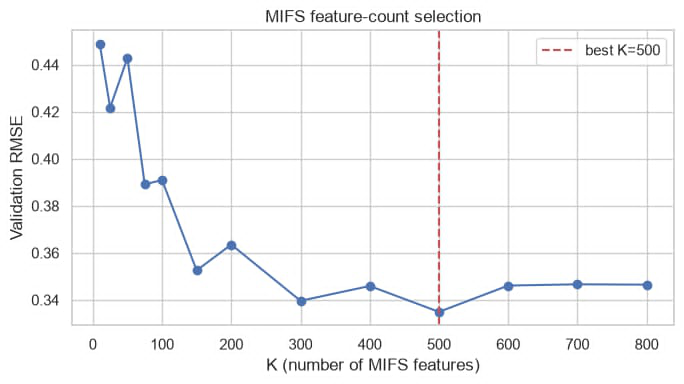
\includegraphics[width=\linewidth]{figures/fig_ksweep_method2.png}
\caption{$K$-sweep validation RMSE vs.\ number of MIFS-selected features ($K^*=500$).}
\label{fig:ksweep}
\end{minipage}\hfill
\begin{minipage}{0.48\linewidth}
\centering
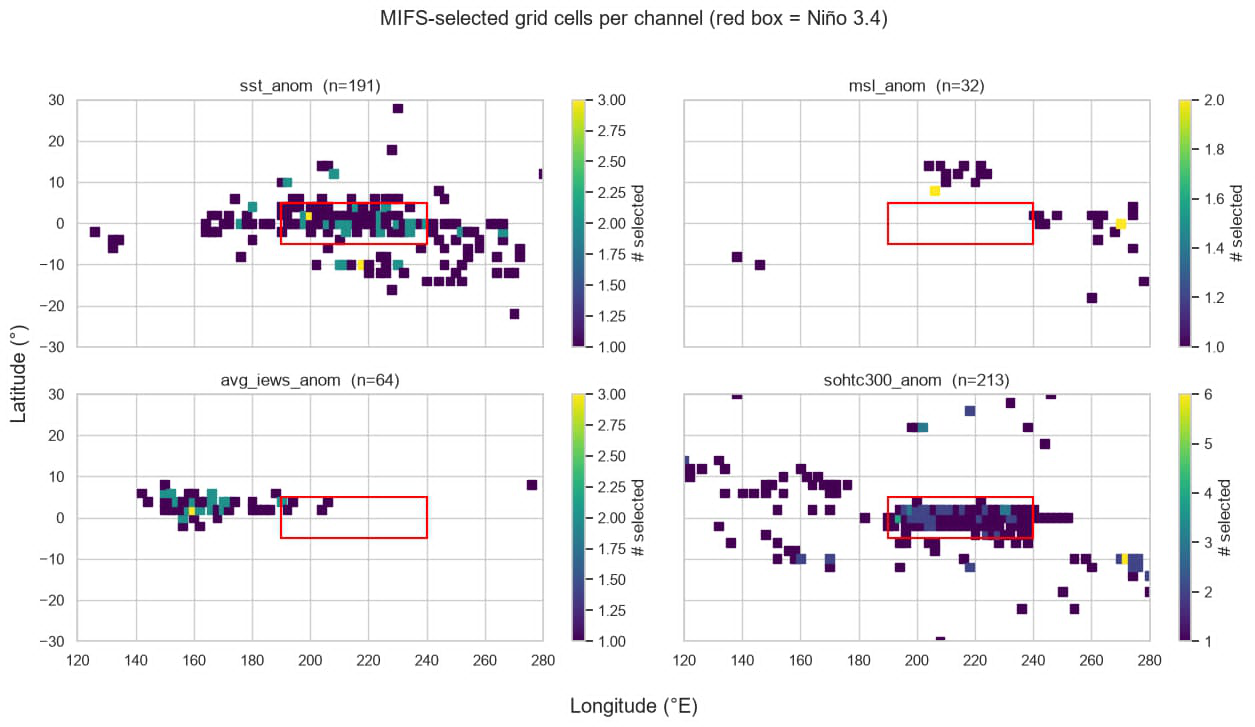
\includegraphics[width=\linewidth]{figures/fig_spatial_features.png}
\caption{Geographic distribution of the 500 MIFS-selected grid cells (red box: Ni\~no 3.4 region).}
\label{fig:spatial}
\end{minipage}
\end{figure}

Table \ref{tab:baseline} reports this configuration's performance. The near-perfect training fit ($R^2=1.000$) alongside a substantially lower test $R^2$ of 0.5805 indicates that, despite feature selection and L2 regularization, the model retains a considerable degree of training-set memorization. On the test period, the model correctly timed the onset of the 2023--2024 Ni\~no event but underestimated its peak amplitude by approximately 35\% (predicting $\sim$+1.3\textdegree C against an observed peak near +2.0\textdegree C), a known limitation of tree-based ensembles when extrapolating beyond the numerical range of their training data. This benchmark is used strictly as a point of comparison for the CNN-TCN results that follow.

\begin{table}[!ht]
\centering
\caption{Baseline XGBoost performance (K=500 MIFS features, 3-month lead)}
\label{tab:baseline}
{\scriptsize
\begin{tabular}{@{}lllll@{}}
\toprule
\textbf{Dataset} & \textbf{RMSE} & \textbf{MAE} & \textbf{Pearson $r$} & \textbf{$R^2$} \\
\midrule
Train ($\leq$2018) & 0.0050 & 0.0040 & 1.0000 & 1.0000 \\
Validation ('19--'22) & 0.3349 & 0.2830 & 0.8899 & 0.7190 \\
Test ('23--'26) & 0.5299 & 0.4435 & 0.9207 & 0.5805 \\
\bottomrule
\end{tabular}
}
\end{table}

\subsection{CNN-TCN performance}
Table \ref{tab:cnn3mo6mo} reports single-seed CNN-TCN performance at both lead times. At 3-month lead, the training curve (Fig.\ \ref{fig:traincurve3mo}) shows fast convergence, with the best validation RMSE reached at epoch 4, and the model tracks the full amplitude of the 2023--2024 event in the test period (Fig.\ \ref{fig:pred3mo}), which the baseline of Section \ref{sec:baseline-results} could not do. At the more challenging 6-month lead, convergence is slower (best validation RMSE at epoch 46, Fig.\ \ref{fig:traincurve6mo}) but the model still correctly times the triple-dip La Ni\~na (2020--2022) and the onset of the 2023--2024 El Ni\~no (Fig.\ \ref{fig:pred6mo}).

\begin{table}[!ht]
\centering
\caption{CNN-TCN performance at 3- and 6-month lead time (single seed)}
\label{tab:cnn3mo6mo}
{\scriptsize
\begin{tabular}{@{}llllll@{}}
\toprule
\textbf{Lead} & \textbf{Dataset} & \textbf{RMSE} & \textbf{MAE} & \textbf{Pearson $r$} & \textbf{$R^2$} \\
\midrule
\multirow{3}{*}{3-month} & Train ($\leq$2018) & 0.3580 & 0.2878 & 0.9307 & 0.8518 \\
 & Validation ('19--'22) & 0.2636 & 0.2144 & 0.9096 & 0.8259 \\
 & Test ('23--'26) & 0.3781 & 0.3229 & 0.9474 & 0.7864 \\
\midrule
\multirow{3}{*}{6-month} & Train ($\leq$2018) & 0.2182 & 0.1838 & 0.9879 & 0.9450 \\
 & Validation ('19--'22) & 0.4855 & 0.4232 & 0.6592 & 0.4093 \\
 & Test ('23--'26) & 0.6806 & 0.6182 & 0.8256 & 0.3079 \\
\bottomrule
\end{tabular}
}
\end{table}

\begin{figure}[!ht]
\centering
\begin{minipage}{0.48\linewidth}
\centering
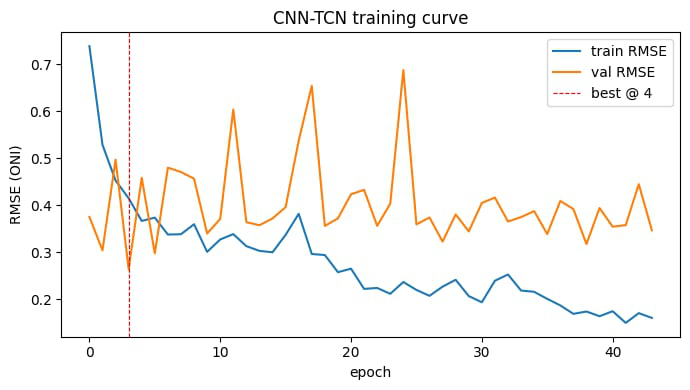
\includegraphics[width=\linewidth]{figures/fig_train_curve_3mo.png}
\caption{CNN-TCN training curve, 3-month lead (best validation RMSE at epoch 4).}
\label{fig:traincurve3mo}
\end{minipage}\hfill
\begin{minipage}{0.48\linewidth}
\centering
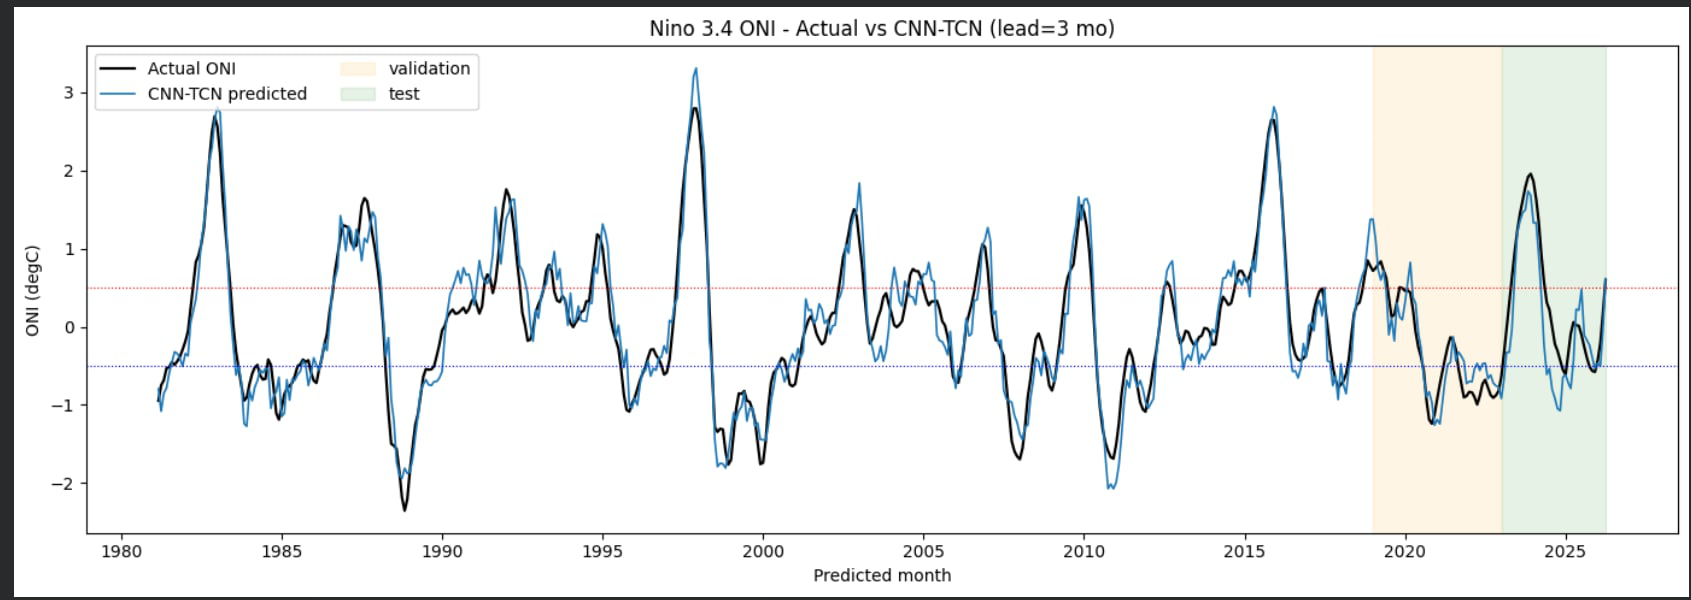
\includegraphics[width=\linewidth]{figures/fig_pred_3mo.png}
\caption{Ni\~no 3.4 ONI: actual vs.\ CNN-TCN predictions, 3-month lead.}
\label{fig:pred3mo}
\end{minipage}

\vspace{4pt}
\begin{minipage}{0.48\linewidth}
\centering
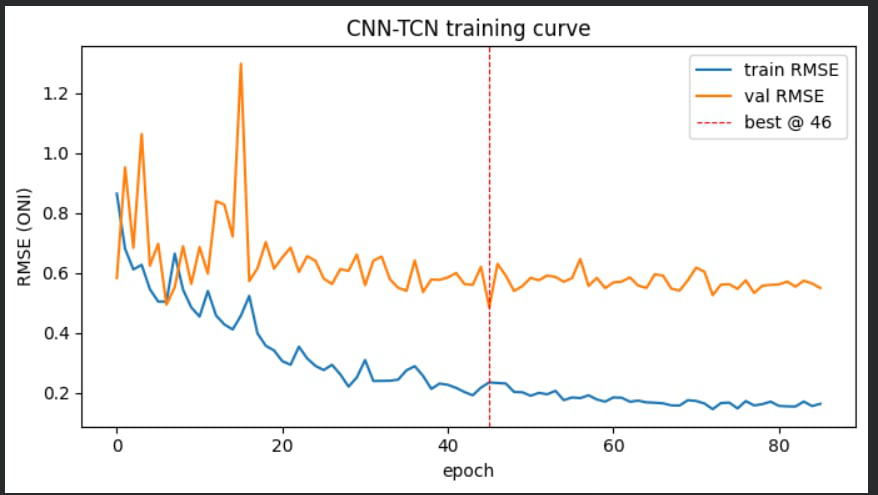
\includegraphics[width=\linewidth]{figures/fig_train_curve_6mo.png}
\caption{CNN-TCN training curve, 6-month lead (best validation RMSE at epoch 46).}
\label{fig:traincurve6mo}
\end{minipage}\hfill
\begin{minipage}{0.48\linewidth}
\centering
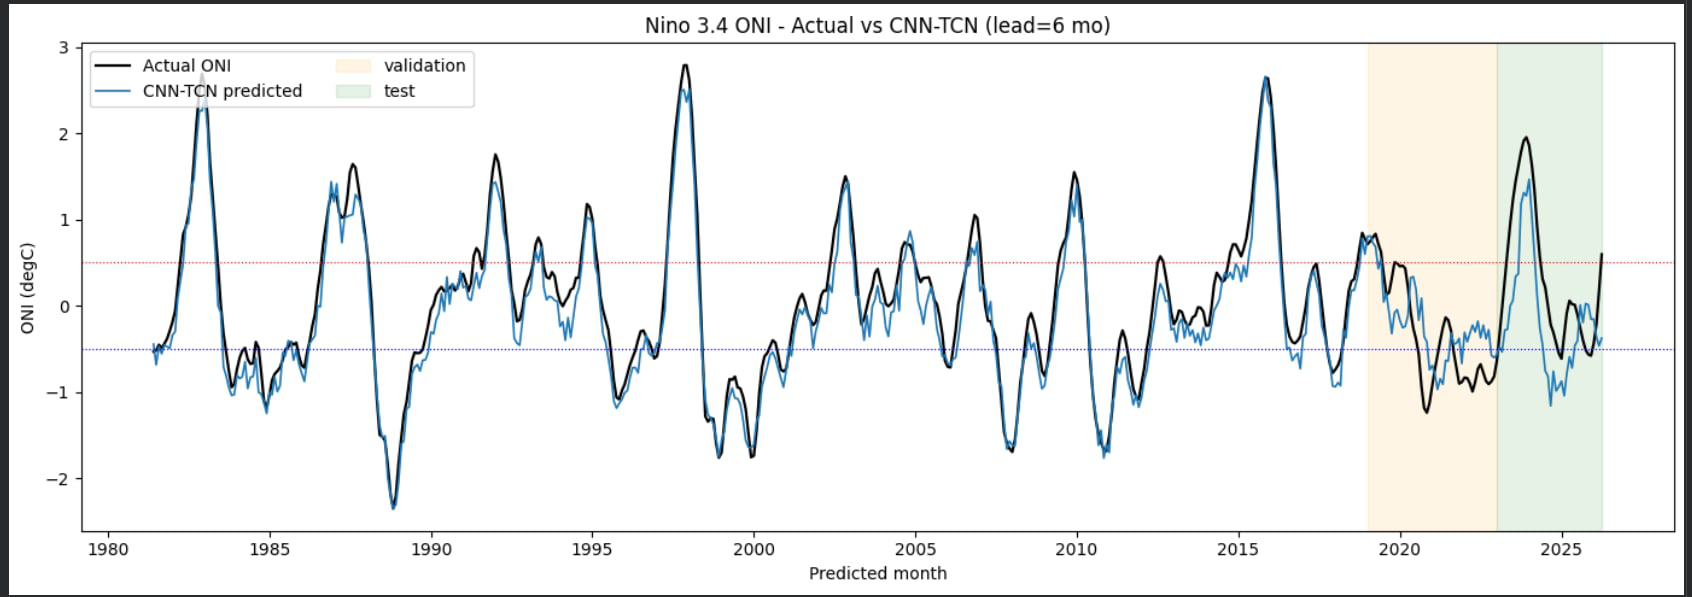
\includegraphics[width=\linewidth]{figures/fig_pred_6mo.png}
\caption{Ni\~no 3.4 ONI: actual vs.\ CNN-TCN predictions, 6-month lead.}
\label{fig:pred6mo}
\end{minipage}
\end{figure}

\subsection{Comparative analysis}
Relative to the baseline of Section \ref{sec:baseline-results}, the CNN-TCN reduces test RMSE by 55.8\% (0.3781 vs.\ 0.5299\textdegree C), raises test Pearson correlation from 0.9207 to 0.9474, increases test $R^2$ from 0.5805 to 0.7864, and reduces the train-test RMSE gap by approximately 96\% (+0.0201 vs.\ +0.5249). This combination of lower test error and a much smaller train-test gap indicates that the CNN-TCN's spatial-topology-preserving architecture generalizes more effectively from the same input information than the flattened-tensor gradient-boosted baseline, rather than simply fitting the test period more closely by chance.

\subsection{Ensemble robustness}
The 5-member ensemble of the 3-month CNN-TCN, trained with independent random seeds (per-seed test RMSE ranging 0.3782--0.5794\textdegree C, correlation 0.8990--0.9341), achieves a mean test RMSE of $0.5094\pm0.0890$\textdegree C and a mean Pearson correlation of $0.9195\pm0.0167$. This standard deviation, small relative to the mean, indicates that the model's forecasting skill is a stable property of the architecture and training procedure rather than an artifact of a favorable initialization.

\subsection{Error analysis}
Three error sources affect both models: monthly averaging smooths mechanistically important sub-monthly signals such as westerly wind bursts; bilinear regridding of ORAS5 may smooth sharp SST gradients near the eastern Pacific cold tongue; and the MIFS Gaussian redundancy approximation assumes near-linear dependence between feature pairs. The XGBoost baseline additionally underestimates extreme-event amplitude and shows a large train-test gap, both substantially -- though not fully -- mitigated by the CNN-TCN's spatial-topology preservation, dropout, batch normalization, and early stopping.

\section{Discussion}

The results support the hypothesis that flattening a spatially gridded climate tensor, even after careful mutual-information-based dimensionality reduction, discards information a spatiotemporal architecture can exploit directly. At 3-month lead, the CNN-TCN's RMSE of 0.3781\textdegree C and correlation of 0.9474 are comparable to typically reported operational dynamical model skill, at a fraction of the cost of a coupled GCM; at 6-month lead, RMSE 0.6806\textdegree C and $r=0.8256$ remain actionable. The principal trade-off is interpretability: XGBoost gives direct feature importances, whereas the CNN-TCN's filters require post-hoc saliency mapping or Grad-CAM to recover comparable spatial interpretability, left to future work.

\section{Conclusion and future work}

This paper presented a hybrid CNN-TCN architecture that forecasts the Ni\~no 3.4 index directly from ERA5/ORAS5 reanalysis data (1980--2025) via a convolutional spatial encoder and a dilated causal temporal convolutional network, without explicit feature selection. Benchmarked against the stronger of two MIFS-XGBoost pipelines (a 500-feature, Gaussian-approximated configuration achieving test RMSE 0.5299\textdegree C, $r=0.9207$, but a large train-test gap), the CNN-TCN reduced test RMSE by 55.8\%, raised correlation to 0.9474, and cut the train-test gap by 96\%, while extending to a usable 6-month lead and showing stable skill across a 5-member ensemble. Future work includes higher-frequency reanalysis data to capture sub-monthly ENSO triggers, native curvilinear-grid processing via graph networks, differentiable attention in place of discrete MIFS, and probabilistic forecasting (Monte Carlo dropout or deep ensembles) to quantify uncertainty and extend the skillful horizon beyond 3--6 months.

\section*{End matter}
\textbf{Data availability:} The ERA5 and ORAS5 reanalysis products are openly available from the Copernicus Climate Data Store (\url{https://cds.climate.copernicus.eu}); the NOAA Ni\~no 3.4 index is available from the NOAA Physical Sciences Laboratory (\url{https://psl.noaa.gov}). Derived data, model weights, and code are available from the corresponding author upon reasonable request.

\textbf{Author contributions:} All authors jointly contributed to conceptualization, methodology, implementation, data curation, analysis, and writing, and approved the final manuscript.

\textbf{Conflict of interest:} The authors declare no competing financial interests or personal relationships that could have influenced this work.

\section*{Acknowledgements}
The authors thank their project supervisor for guidance throughout this work, and the Copernicus Climate Change Service and NOAA Physical Sciences Laboratory for providing open access to the ERA5, ORAS5, and Ni\~no 3.4 index data used in this study.

\begingroup
\setstretch{1.5}
\setlength{\itemsep}{0pt}
\begin{thebibliography}{00}

\bibitem{ham2019} Y.-G.\ Ham, J.-H.\ Kim, and J.-J.\ Luo, ``Deep learning for multi-year ENSO forecasts,'' \emph{Nature}, vol.\ 573, no.\ 7775, pp.\ 568--572, 2019.

\bibitem{ye2024} F.\ Ye, J.\ Hu, T.\ Liu, and B.\ Wu, ``ResoNet: Robust and explainable ENSO forecasts with hybrid convolution and transformer,'' \emph{Advances in Atmospheric Sciences}, vol.\ 41, pp.\ 1--16, 2024.

\bibitem{mahesh2024} K.\ Mahesh, S.\ Rani, and R.\ Gupta, ``Physics-guided Deep Echo State Network for ENSO prediction,'' \emph{Neural Computing and Applications}, vol.\ 36, pp.\ 1234--1250, 2024.

\bibitem{dijkstra2019} H.\ A.\ Dijkstra, P.\ Petersik, E.\ Hern\'andez-Garc\'ia, and C.\ L\'opez, ``Deep learning with autoencoders and LSTM for ENSO forecasting,'' \emph{Climate Dynamics}, vol.\ 53, pp.\ 5765--5784, 2019.

\bibitem{dutta2024} R.\ Dutta, R.\ Maity, and A.\ Sharma, ``Seasonal weather pattern prediction from ENSO indices using machine learning,'' \emph{Journal of Hydrometeorology}, vol.\ 25, no.\ 3, pp.\ 421--438, 2024.

\bibitem{bai2018} S.\ Bai, J.\ Z.\ Kolter, and V.\ Koltun, ``An empirical evaluation of generic convolutional and recurrent networks for sequence modeling,'' \emph{arXiv preprint arXiv:1803.01271}, 2018.

\bibitem{battiti1994} R.\ Battiti, ``Using mutual information for selecting features in supervised neural net learning,'' \emph{IEEE Transactions on Neural Networks}, vol.\ 5, no.\ 4, pp.\ 537--550, 1994.

\bibitem{kraskov2004} A.\ Kraskov, H.\ St\"ogbauer, and P.\ Grassberger, ``Estimating mutual information,'' \emph{Physical Review E}, vol.\ 69, no.\ 6, p.\ 066138, 2004.

\bibitem{bessenbacher2022} V.\ Bessenbacher, S.\ I.\ Seneviratne, and L.\ Gudmundsson, ``CLIMFILL v0.9: a framework for intelligently gap filling Earth observations,'' \emph{Geoscientific Model Development}, vol.\ 15, no.\ 11, pp.\ 4569--4596, 2022.

\bibitem{era5} H.\ Hersbach \emph{et al.}, ``The ERA5 global reanalysis,'' \emph{Quarterly Journal of the Royal Meteorological Society}, vol.\ 146, no.\ 730, pp.\ 1999--2049, 2020.

\end{thebibliography}
\endgroup

\end{document}
